% S02-T1: BG(U_1(5),2) for B_3 and its covering by T_2.  math: plan/staged/stage-02-tree-quotients.tex  def:s02-BG, prop:s02-quot
% data: code/results/s02/T3.json (U_1(5), self_contained_graph), S02-C3
\begin{frame}{A concrete quotient: $\mathrm{BG}(U_1(5),2)$ for $B_3$ ($D=3$)}
  \centering
  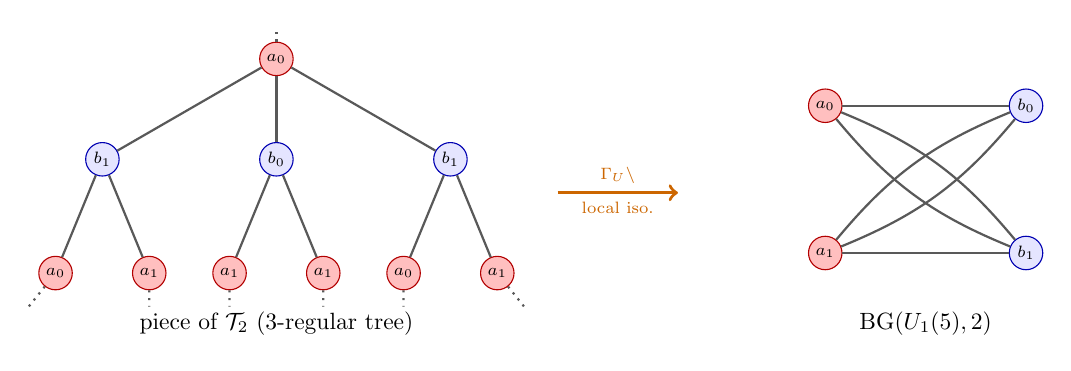
\begin{tikzpicture}[scale=0.85,transform shape,
      every node/.style={font=\scriptsize},
      va/.style={circle,draw=red!70!black,fill=red!25,inner sep=1.2pt,minimum size=5mm},
      vb/.style={circle,draw=blue!70!black,fill=blue!10,inner sep=1.2pt,minimum size=5mm},
      ed/.style={thick,gray!70!black}]
    % ---- piece of the 3-regular tree T_2, radius 2 around a type-0 vertex ----
    \node[va] (r) at (0,1.9) {$a_0$};
    \node[vb] (c1) at (-2.6,0.4) {$b_1$};
    \node[vb] (c2) at (0,0.4) {$b_0$};
    \node[vb] (c3) at (2.6,0.4) {$b_1$};
    \node[va] (g1) at (-3.3,-1.3) {$a_0$};
    \node[va] (g2) at (-1.9,-1.3) {$a_1$};
    \node[va] (g3) at (-0.7,-1.3) {$a_1$};
    \node[va] (g4) at (0.7,-1.3) {$a_1$};
    \node[va] (g5) at (1.9,-1.3) {$a_0$};
    \node[va] (g6) at (3.3,-1.3) {$a_1$};
    \foreach \p/\c in {r/c1,r/c2,r/c3,c1/g1,c1/g2,c2/g3,c2/g4,c3/g5,c3/g6}
      \draw[ed] (\p) -- (\c);
    \foreach \c/\dx in {g1/-0.5,g2/0,g3/0,g4/0,g5/0,g6/0.5}
      \draw[ed,dotted] (\c) -- ++(\dx-0.2*\dx,-0.5) ;
    \draw[ed,dotted] (r) -- ++(0,0.45);
    \node at (0,-2.05) {\normalsize piece of $\mathcal T_2$ (3-regular tree)};
    % ---- covering map ----
    \draw[->,very thick,orange!80!black] (4.2,-0.1) -- node[above] {$\Gamma_U\backslash$} node[below] {local iso.} (6.0,-0.1);
    % ---- BG(U_1(5),2) ----
    \begin{scope}[shift={(8.2,0)}]
      \node[va] (a0) at (0,1.2) {$a_0$};
      \node[va] (a1) at (0,-1.0) {$a_1$};
      \node[vb] (b0) at (3,1.2) {$b_0$};
      \node[vb] (b1) at (3,-1.0) {$b_1$};
      \draw[ed] (a0) -- (b0);
      \draw[ed] (a1) -- (b1);
      \draw[ed] (a0) to[bend left=14] (b1);
      \draw[ed] (a0) to[bend right=14] (b1);
      \draw[ed] (a1) to[bend left=14] (b0);
      \draw[ed] (a1) to[bend right=14] (b0);
      \node at (1.5,-2.05) {\normalsize $\mathrm{BG}(U_1(5),2)$};
    \end{scope}
  \end{tikzpicture}

  \vspace{-1mm}
  \begin{itemize}\small
    \item $2+2$ vertices (types $0,1$), $6$ edges; $\operatorname{rank}H_1=6-4+1=3$ (genus $3$ in \texttt{T3.json}).
    \item Edge multiplicities: $a_0b_0:1,\ a_0b_1:2,\ a_1b_0:2,\ a_1b_1:1$.
      Every vertex has degree $q+1=3$; the labels on the tree show the covering map locally.
  \end{itemize}
  \vfill
  {\tiny Sources: \texttt{code/results/s02/T3.json} (entry $U_1(5)$, \texttt{self\_contained\_graph}, S02-C3);
  \texttt{def:s02-BG}, \texttt{prop:s02-quot} in \texttt{plan/staged/stage-02-tree-quotients.tex}; status: computed.}
\end{frame}
